\section{图像分割问题}
\begin{frame}[allowframebreaks]
  \frametitle{\textsc{目录}} \vspace{-0.3cm}
    \begin{spacing}{0.0}
        \tableofcontents[currentsection,hideallsubsections]
    \end{spacing}   % 若不想要目录, 注释掉该句
\end{frame}



\begin{frame}
    \noindent\large\textbf{图像分割问题}

    \vspace{1em}
    图像分割任务:将完整图像分割成若干互不重叠的子区域

    \vspace{0.1em}
    从机器学习的角度来说,图像分割是为图像中的每一个像素点分配一个标签

    \vspace{0.1em}
    图像分割又分为语义分割(semantic segmentation)和实例分割(instance segmentation)
    \begin{figure}
        \subfloat[语义分割]{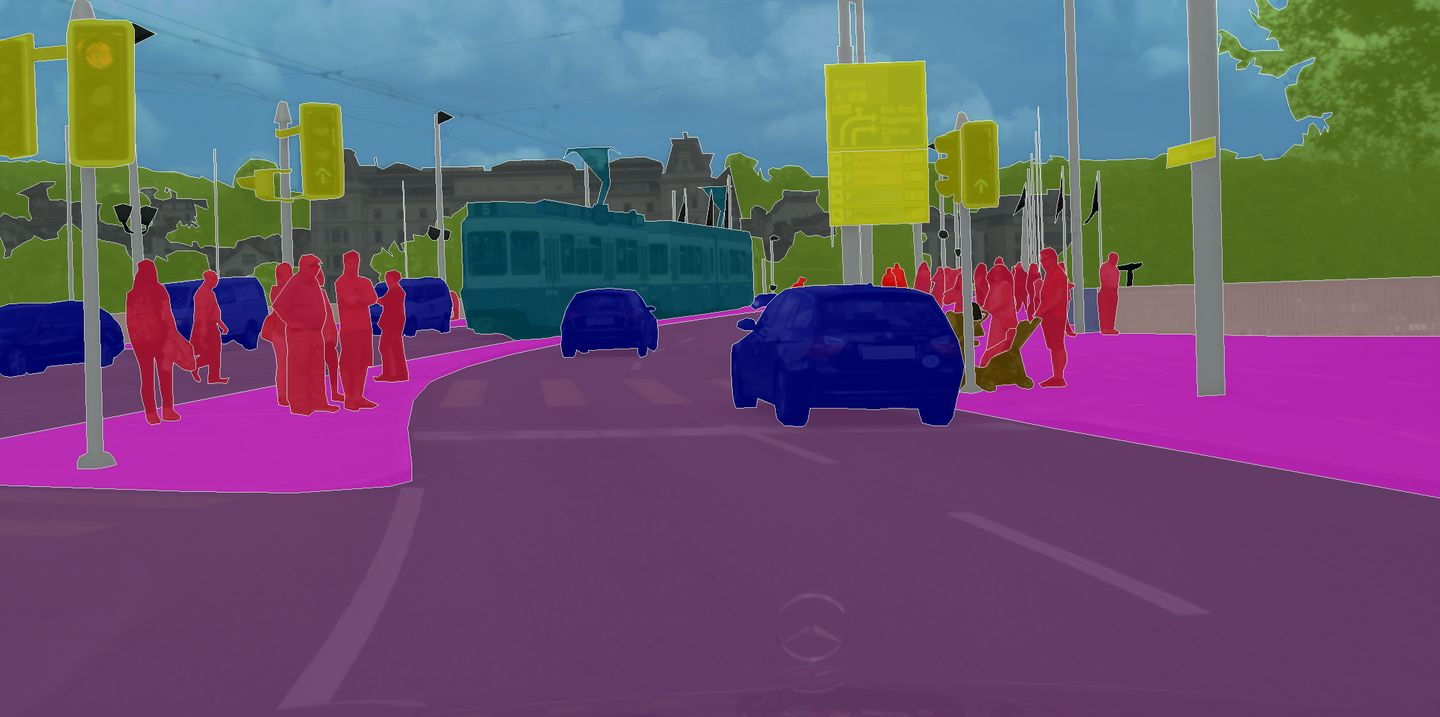
\includegraphics[width=5.5cm,height=3cm]{2.jpg}}
        \subfloat[实例分割]{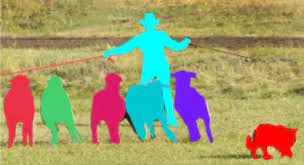
\includegraphics[width=5.5cm,height=3cm]{3.jpeg}}
    \end{figure}
\end{frame}

\begin{frame}
    \noindent\large\textbf{标签}

    \vspace{0.1em}
    语义分割:所属的物体的类别

    \vspace{0.1em}
    实例分割:所属对象的编号

    \begin{figure}
        \subfloat[类别标签]{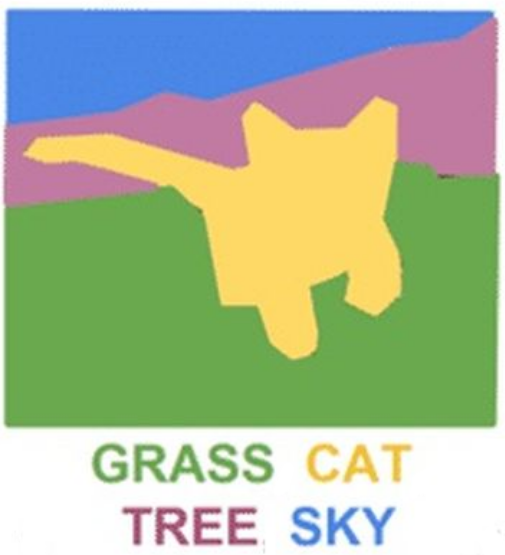
\includegraphics[width=3.6cm,height=4.4cm]{4.png}}
        \subfloat[对象标签]{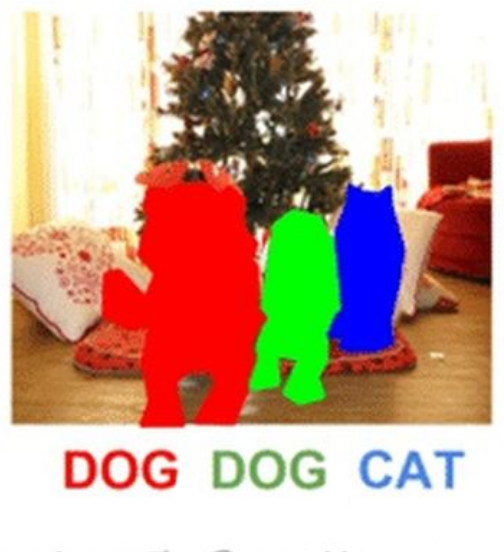
\includegraphics[width=3.4cm,height=4.4cm]{5.png}}
    \end{figure}

    实例分割$\approx $目标检测$+$语义分割
\end{frame}

\begin{frame}
    \noindent\large\textbf{数据}

    \begin{itemize}
    \item[$ \bullet $]  包含图像和标签(掩码、mask、Ground Truth)

    %\vspace{1em}
    \item[$ \bullet $]  图像与标签大小相同

    %\vspace{1em}
    \item[$ \bullet $]  图像与标签的像素一一对应

    %\vspace{1em}
    \item[$ \bullet $] 标签的形式多种多样,包括图像、描述文件、表格等形式
    \end{itemize}

    \vspace{1em}
        \begin{figure}
        \subfloat[mask]{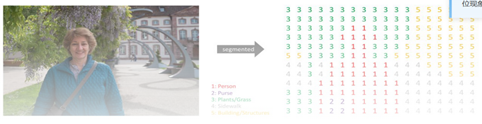
\includegraphics[width=0.9\linewidth]{mask.png}}
    \end{figure}

 %   \noindent\large\textbf{常见数据集}
%
%    \vspace{1em} \small
%    Common Objects in COntext(COCO)、PASCAL Visual Object Classes(PASAL)、
%    The Cityscapes Dataset、The Cambridge-driving Labeled Video Database(CamVid)、
%    Stanford Background Dataset、Barcelona Dataset、Microsoft Research in Cambridge、
%    LITS Liver Tumor Segmentation Dataset、ISBI Challenge
\end{frame}


\begin{frame}
    \noindent\large\textbf{常见数据集}

%    \begin{itemize}
%    \item[$ \bullet $]  包含图像和标签(掩码、mask、Ground Truth)
%
%    %\vspace{1em}
%    \item[$ \bullet $]  图像与标签大小相同
%
%    %\vspace{1em}
%    \item[$ \bullet $]  图像与标签的像素一一对应
%
%    %\vspace{1em}
%    \item[$ \bullet $] 标签的形式多种多样,包括图像、描述文件、表格等形式
%    \end{itemize}
%
%    \vspace{1em}
%    \noindent\large\textbf{常见数据集}

    \vspace{1em} \small
    Common Objects in COntext(COCO)、PASCAL Visual Object Classes(PASAL)、
    The Cityscapes Dataset、The Cambridge-driving Labeled Video Database(CamVid)、
    Stanford Background Dataset、Barcelona Dataset、Microsoft Research in Cambridge、
    LITS Liver Tumor Segmentation Dataset、ISBI Challenge
\end{frame}



\begin{frame}
    \noindent\large\textbf{常用评价指标}

    \vspace{0.1em}
    $\bullet$ 准确率:$PA=\frac{TP+TN}{TP+FP+FN+TN}$

    \vspace{0.1em}
    $\bullet$ Dice系数(Dice score, F1分数):$dice(A,B)=\frac{2|A\cap B|}{|A|+|B|}=\frac{2TP}{2TP+FN+FP}$

    \vspace{0.1em}
    $\bullet$ 雅卡尔指数(交并比):$IoU=\frac{|A\cap B|}{|A \cup B|} = \frac{TP}{TP + FN + FP}$

    \vspace{0.1em}
    $IoU= \frac{Dice}{2-Dice}$; A: 目标像素的集合;B: 算法判定为目标像素的集合。除此之外还有精确率、召回率、平均准确率、平均精确率、平均召回率和聚合雅卡尔指数等指标

    \begin{figure}
        \subfloat[TP、FP、FN]{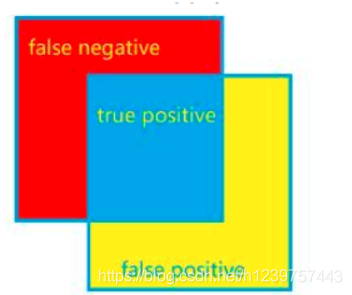
\includegraphics[width=0.3\linewidth]{TPFPFN.png}}
        \subfloat[IoU与Dice]{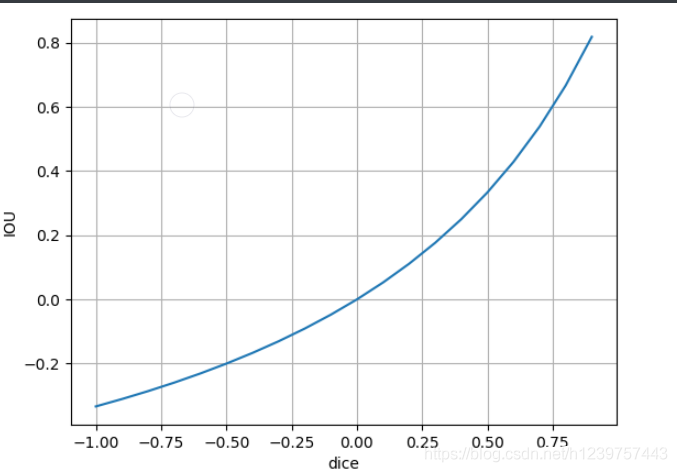
\includegraphics[width=0.3\linewidth]{IoUDice.png}}
    \end{figure}

\end{frame}

\begin{frame}
    \noindent\large\textbf{类别不平衡问题}

    \vspace{1em}
    图像当中的背景与前景常存在像素点数量不平衡的问题,这容易导致模型将所有像素点预测为同一个类别
    \begin{figure}
        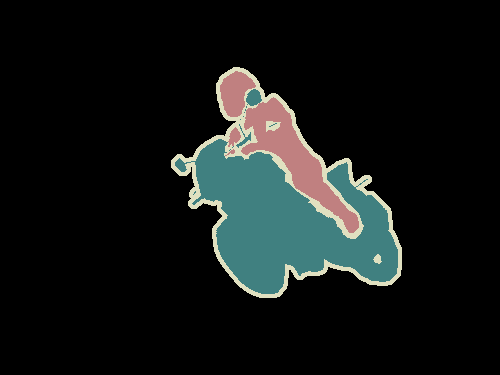
\includegraphics[width=8.0cm]{11.png}
    \end{figure}
\end{frame}

\begin{frame}
    \noindent\large\textbf{解决方法}

    \vspace{1em}
    $\bullet$ 损失函数加权:$L=\sum w_iloss_i$

    \vspace{1em}
    $\bullet$ 欠采样:样本多的类别只统计一部分像素点的损失

    \vspace{1em}
    $\bullet$ Dice损失函数:$L=1-\frac{2\sum \hat{y}_iy_i+\epsilon}{\sum (\hat{y}_i+y_i)+\epsilon}$

    \vspace{1em}
    $\bullet$ Focal损失函数:$L=-\sum (1-\hat{y}_i)^\gamma log(\hat{y}_i)$


\end{frame}

\begin{frame}
    \noindent\large\textbf{图像分割的应用}

    \vspace{1em}
    $\bullet$ 自动驾驶:对周围环境图像进行分割

    \vspace{1em}
    $\bullet$ 医学图像病灶检测:将医学影像当中的病变部位分割出来

    \vspace{1em}
    $\bullet$ 零售图像识别:对货架商品进行监控

    \vspace{1em}
    $\bullet$ 人脸识别:从图像当中提取人脸区域
\end{frame}

